\begin{figure*}[!t]
  \centering

  % 1st row
  \subfloat[\BPNoise~bootstrapped distributions and ranks given by NPSK.]{
    \begin{minipage}{\textwidth}
      % left‐column labels
      \begin{minipage}{0.03\textwidth}
        \footnotesize\raggedleft
        \vspace{0.5cm}
        SIMSE\\[0.6cm]
        L1\\[0.65cm]
        JTFS\\[0.65cm]
        DTW

    % \vspace{-0.2cm} SIMSE\\[0.6cm] L1\\[0.65cm] JTFS\\[0.65cm] DTW %works for full page figures
      \end{minipage}%
      % right‐column images
      \begin{minipage}{0.98\textwidth}\centering
        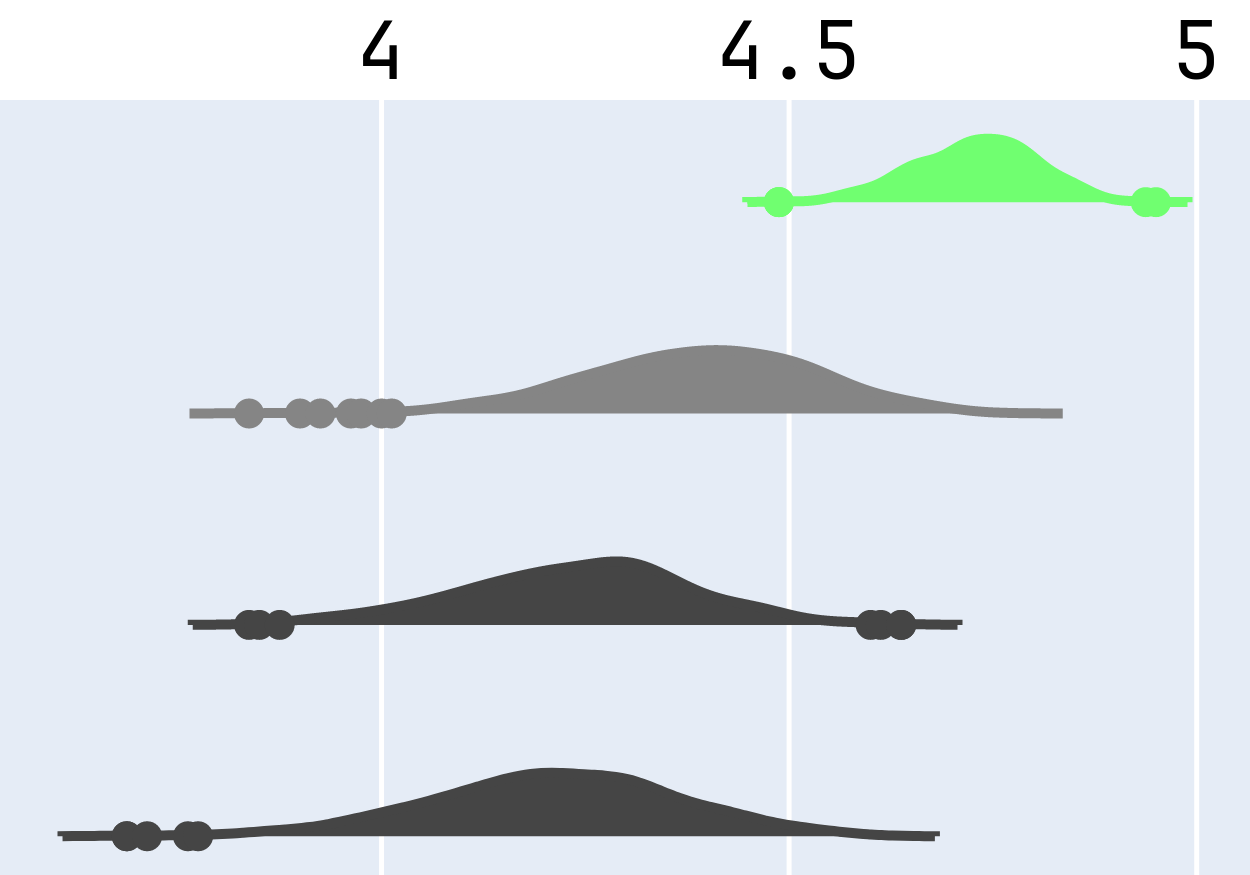
\includegraphics[width=0.31\textwidth]{images/npsk_likert_0.png}%
        \hspace{0.015\textwidth}%
        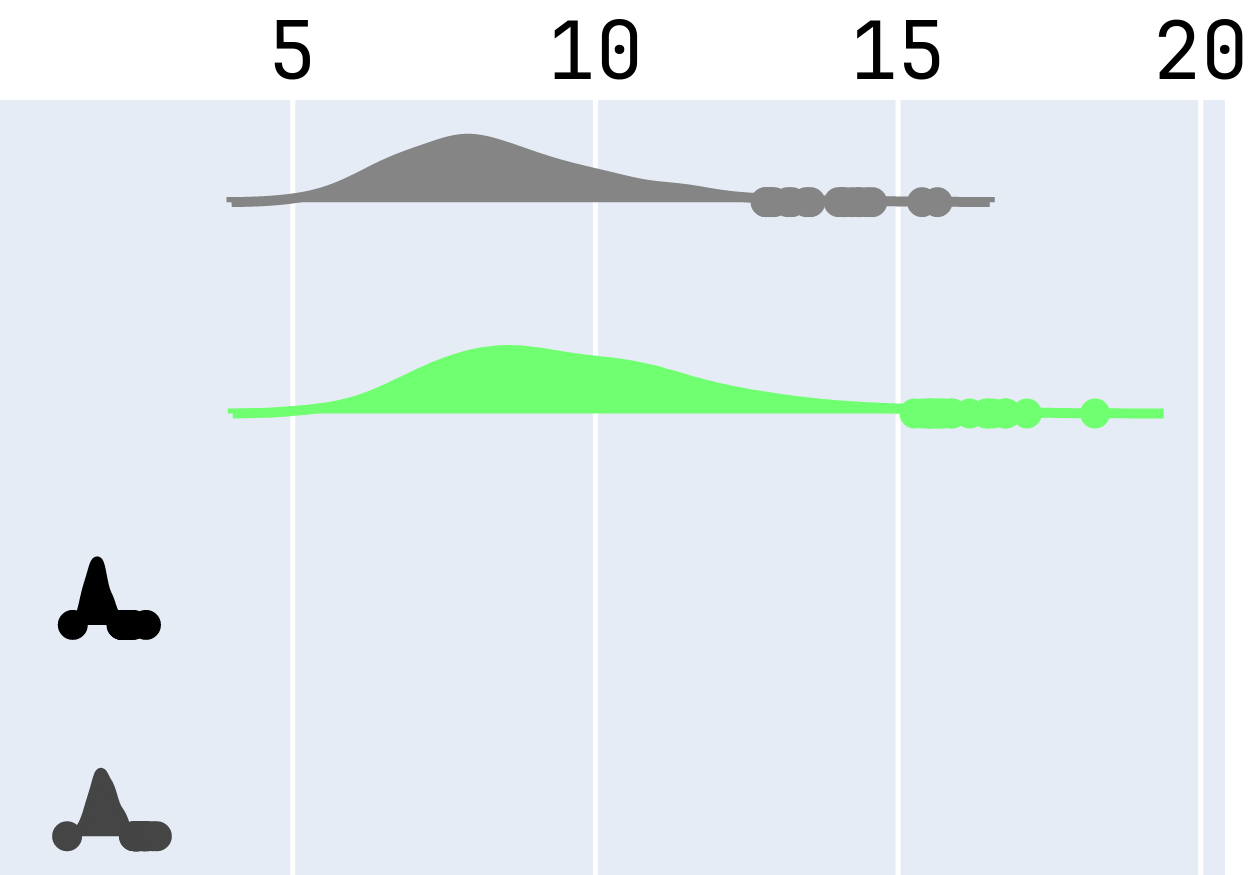
\includegraphics[width=0.31\textwidth]{images/npsk_P-Loss_0.png}%
        \hspace{0.01\textwidth}%
        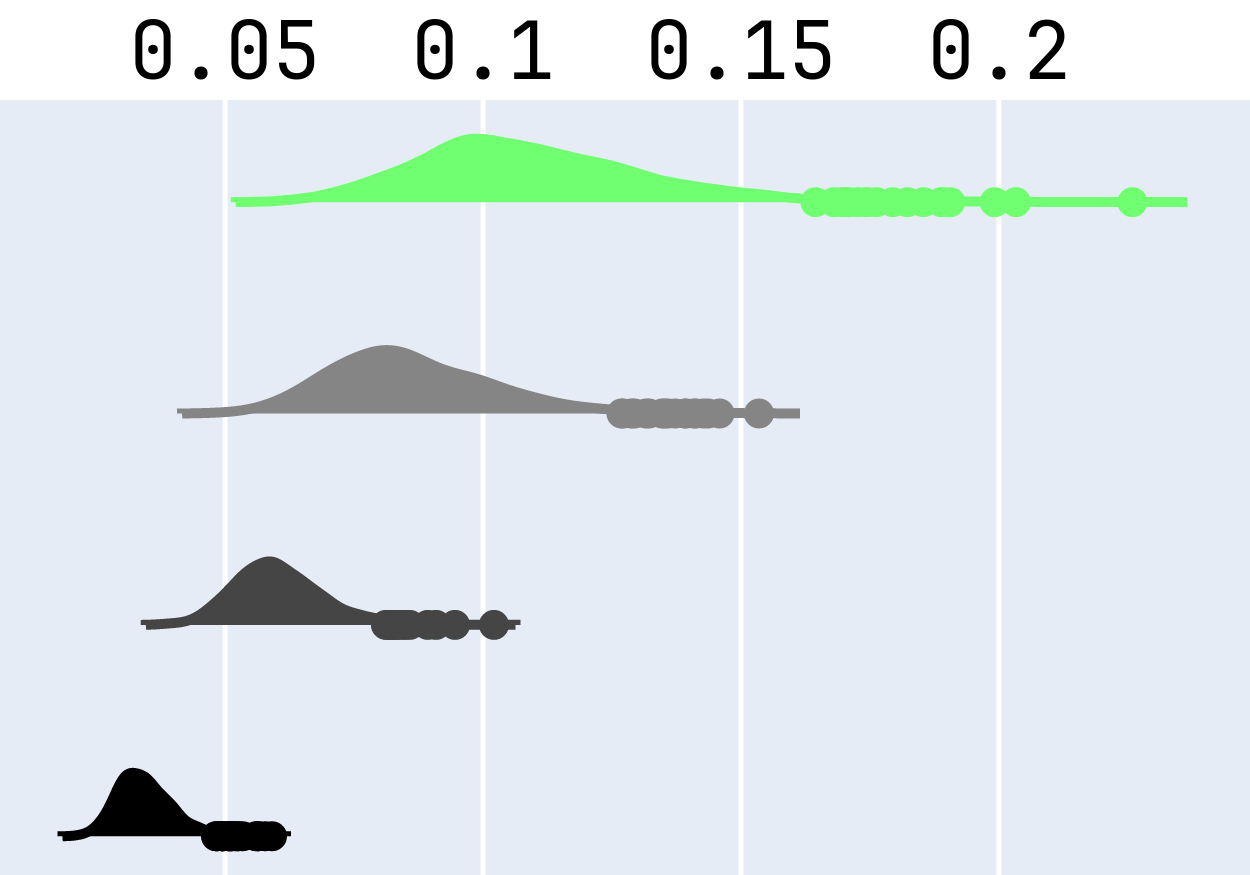
\includegraphics[width=0.31\textwidth]{images/npsk_MSS_0.png}
      \end{minipage}
    \end{minipage}
    \label{fig:npsk_p0}
  }\\[0.5em]  % a bit of vertical space between rows

  % 2nd row
  \subfloat[\AddSineSaw~bootstrapped distributions and ranks given by NPSK.]{
    \begin{minipage}{\textwidth}
      \begin{minipage}{0.03\textwidth}
        \footnotesize\raggedleft
        \vspace{0.5cm}
        SIMSE\\[0.6cm]
        L1\\[0.65cm]
        JTFS\\[0.65cm]
        DTW
      \end{minipage}%
      \begin{minipage}{0.98\textwidth}\centering
        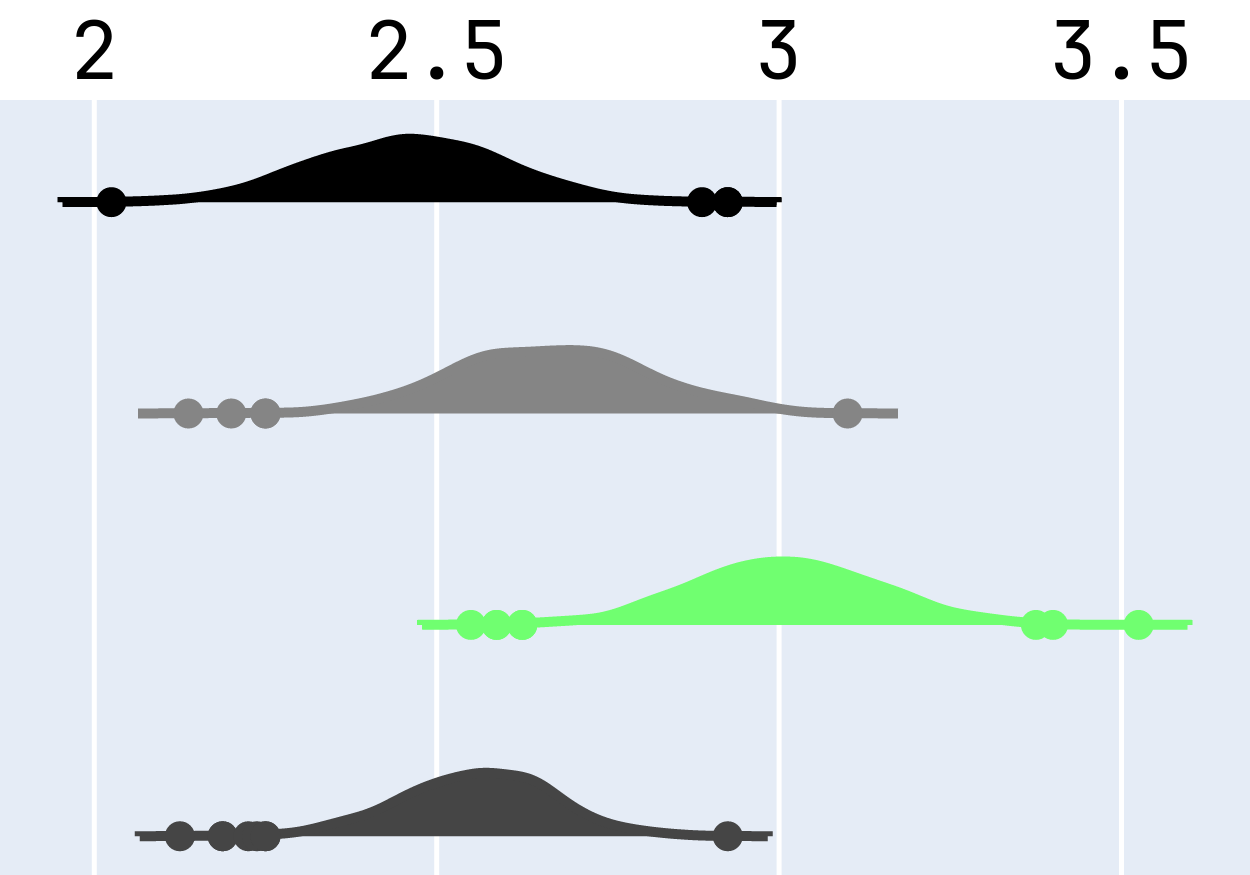
\includegraphics[width=0.31\textwidth]{images/npsk_likert_1.png}%
        \hspace{0.015\textwidth}%
        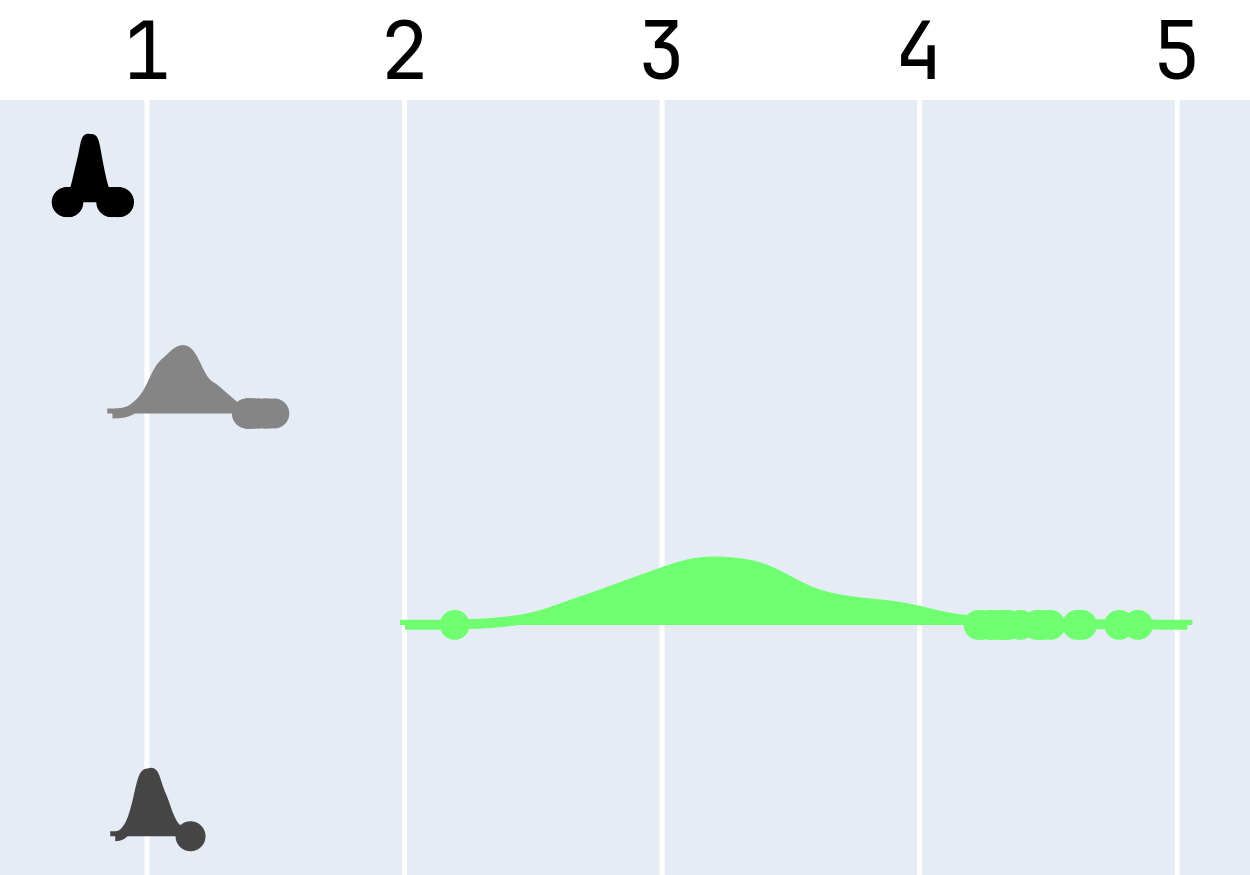
\includegraphics[width=0.31\textwidth]{images/npsk_P-Loss_1.png}%
        \hspace{0.015\textwidth}%
        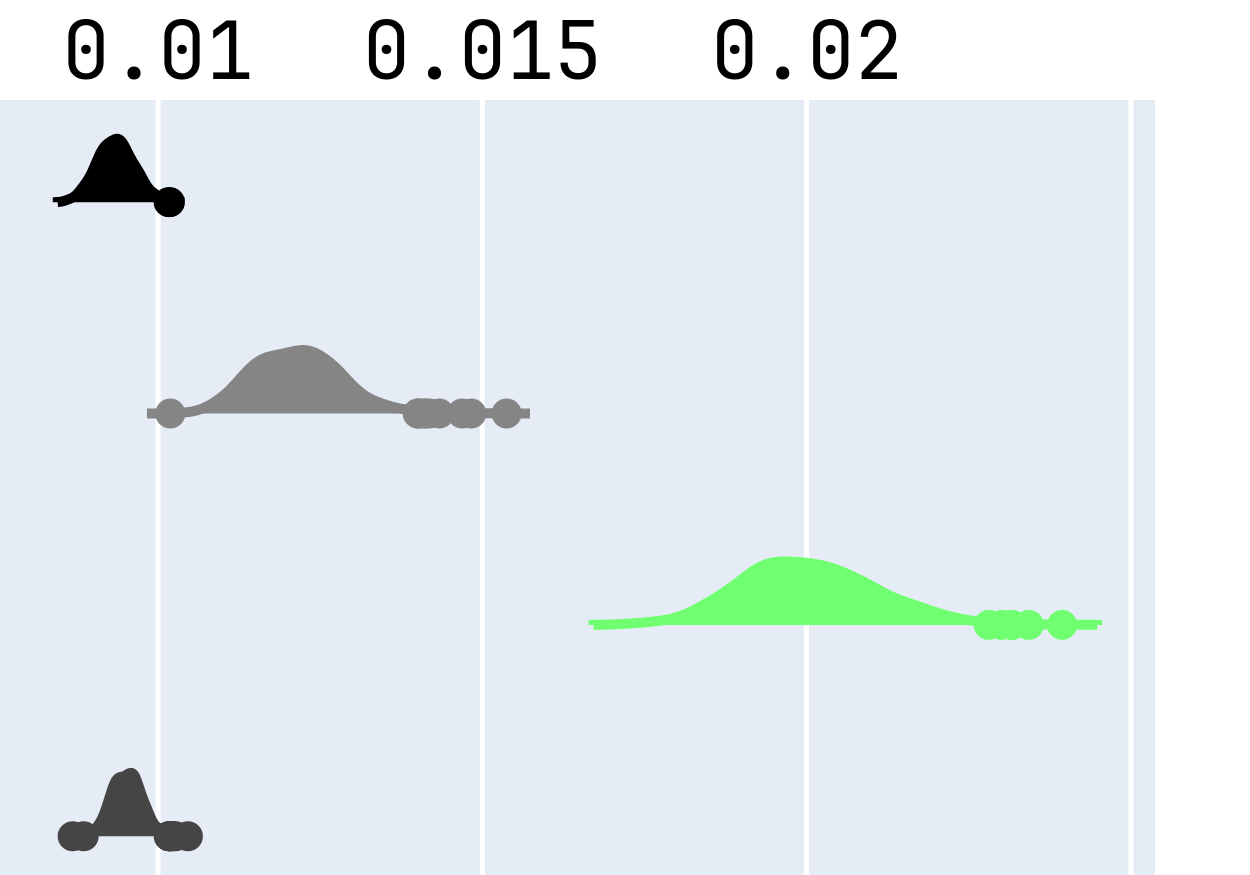
\includegraphics[width=0.31\textwidth]{images/npsk_MSS_1.png}
      \end{minipage}
    \end{minipage}
    \label{fig:npsk_p1}
  }\\[0.5em]

  % 3rd row
  \subfloat[\AmpMod~bootstrapped distributions and ranks given by NPSK.]{
    \begin{minipage}{\textwidth}
      \begin{minipage}{0.03\textwidth}
        \footnotesize\raggedleft
        \vspace{0.5cm}
        SIMSE\\[0.6cm]
        L1\\[0.65cm]
        JTFS\\[0.65cm]
        DTW
      \end{minipage}%
      \begin{minipage}{0.98\textwidth}\centering
        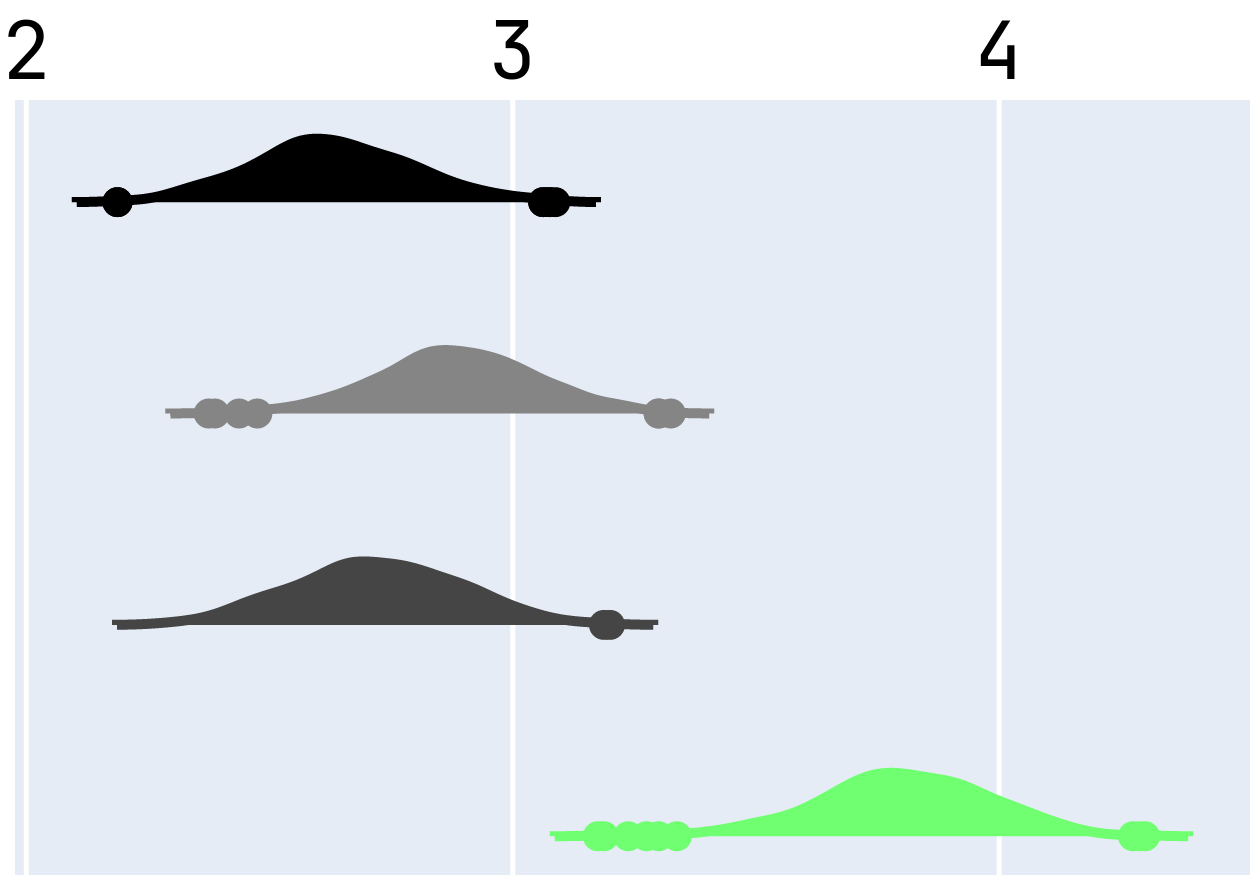
\includegraphics[width=0.31\textwidth]{images/npsk_likert_2.png}%
        \hspace{0.015\textwidth}%
        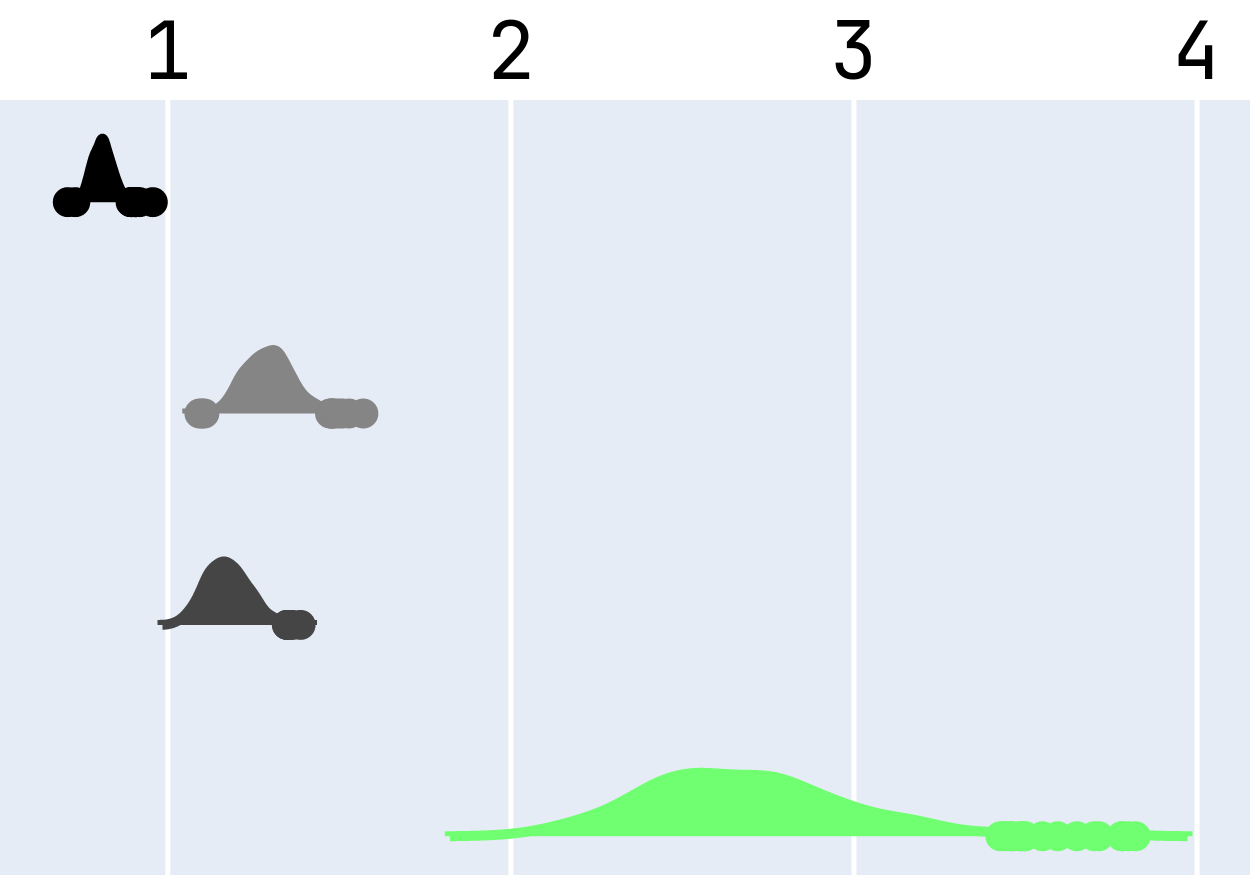
\includegraphics[width=0.31\textwidth]{images/npsk_P-Loss_2.png}%
        \hspace{0.015\textwidth}%
        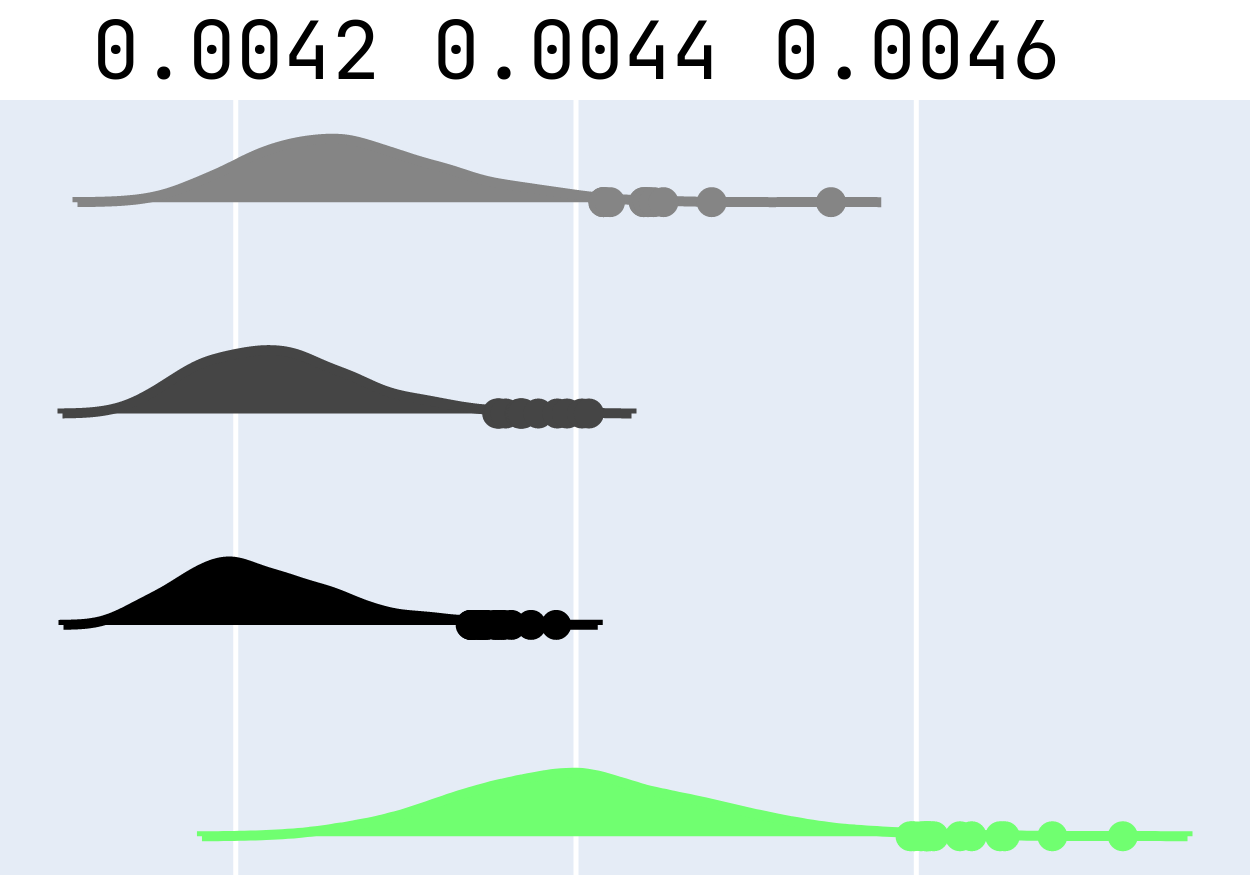
\includegraphics[width=0.31\textwidth]{images/npsk_MSS_2.png}
      \end{minipage}
    \end{minipage}
    \label{fig:npsk_p2}
  }\\[0.5em]

  % 4th row
  \subfloat[\FMMod~bootstrapped distributions and ranks given by NPSK.]{
    \begin{minipage}{\textwidth}
      \begin{minipage}{0.03\textwidth}
        \footnotesize\raggedleft
        \vspace{0.5cm}
        SIMSE\\[0.6cm]
        L1\\[0.65cm]
        JTFS\\[0.65cm]
        DTW
      \end{minipage}%
      \begin{minipage}{0.98\textwidth}\centering
        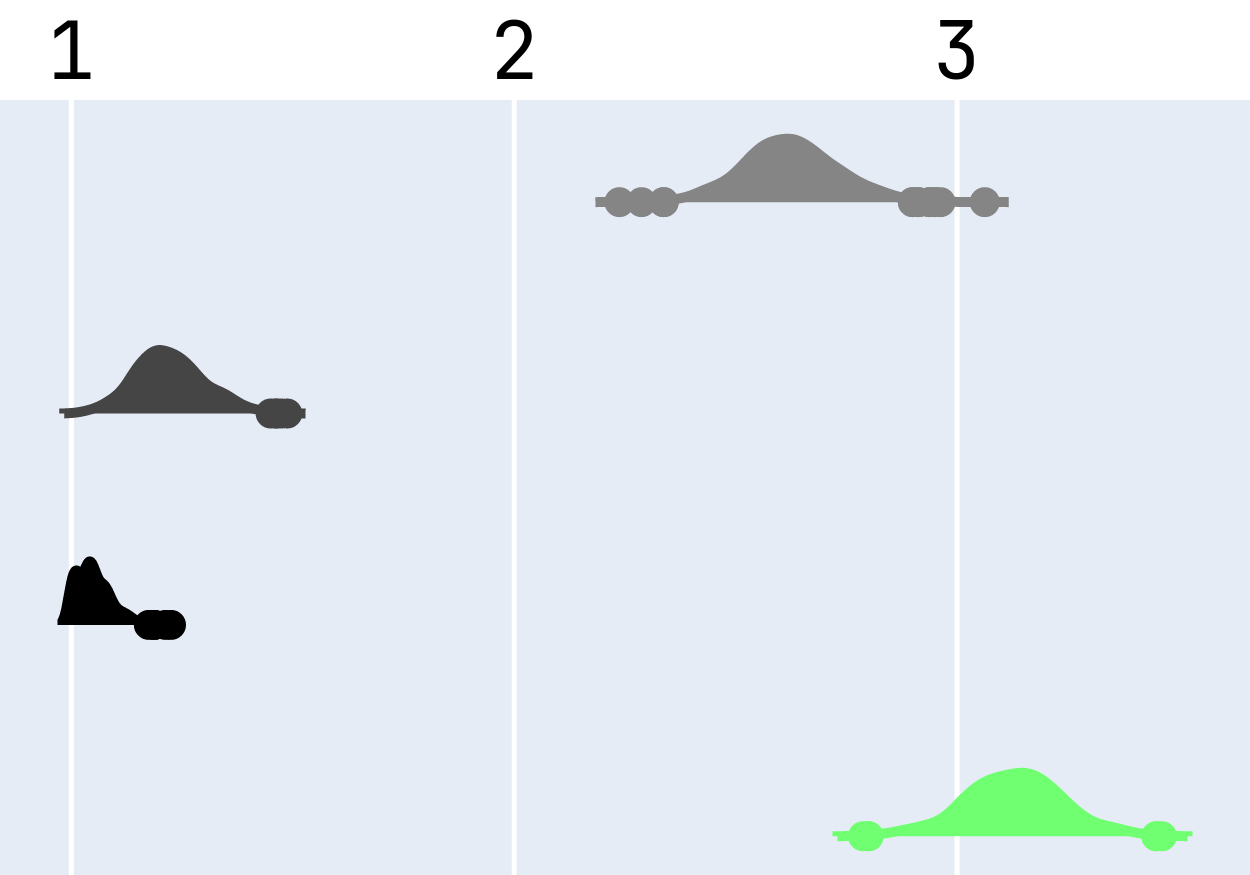
\includegraphics[width=0.31\textwidth]{images/npsk_likert_3.png}%
        \hspace{0.015\textwidth}%
        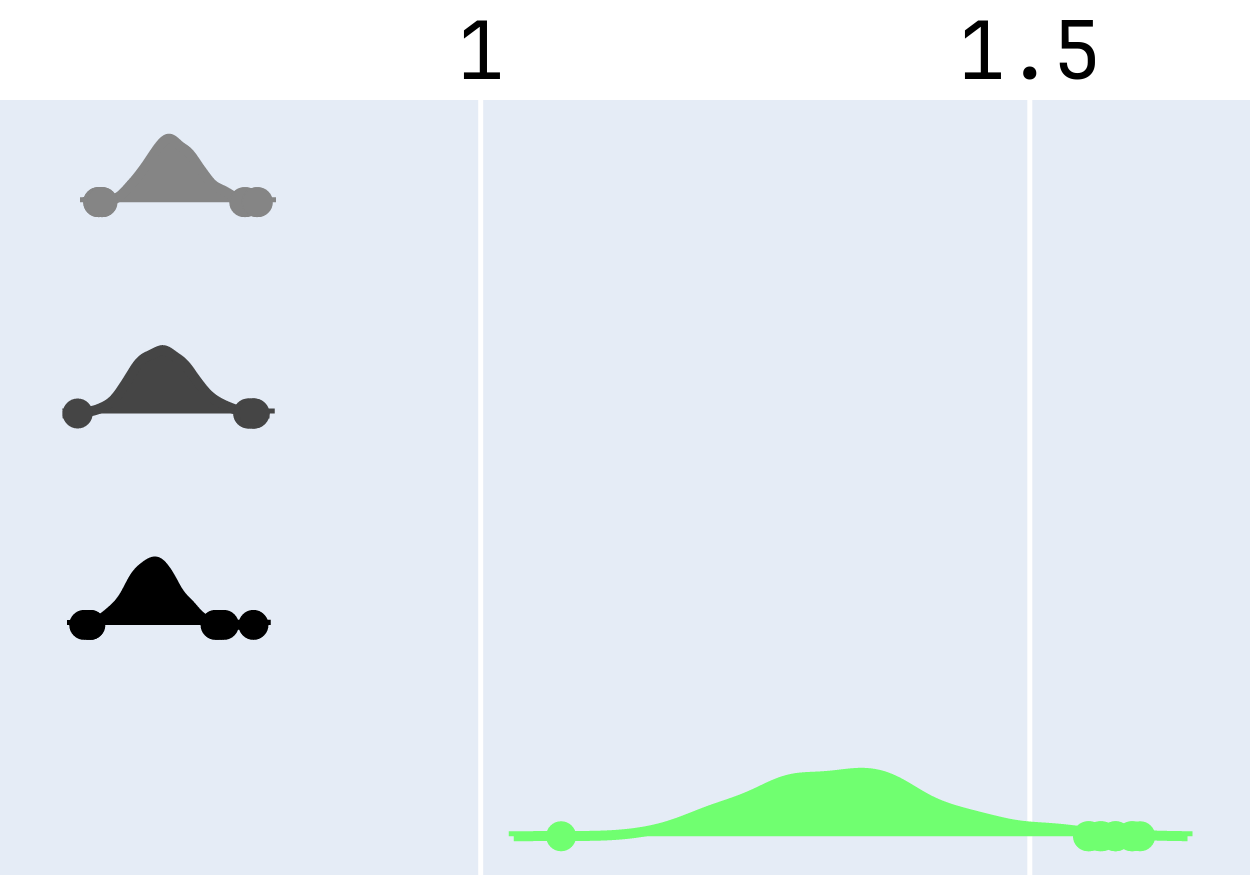
\includegraphics[width=0.31\textwidth]{images/npsk_P-Loss_3.png}%
        \hspace{0.015\textwidth}%
        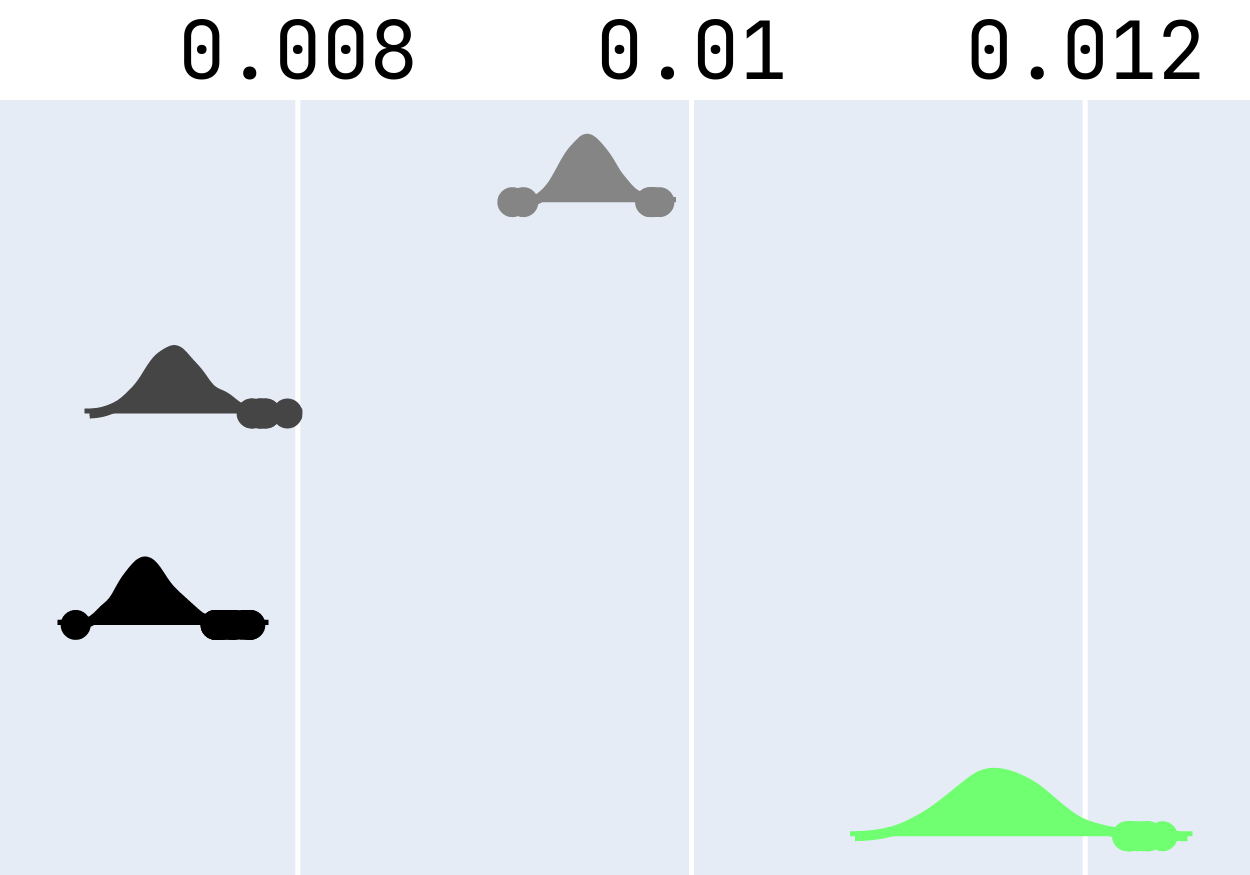
\includegraphics[width=0.31\textwidth]{images/npsk_MSS_3.png}
      \end{minipage}
    \end{minipage}
    \label{fig:npsk_p3}
  }

  \caption{Higher values indicate better performance. Rank colors are
\colorbox{rank1}{\textcolor{black}{\textbf{1}}} \colorbox{rank2}{\textcolor{white}{\textbf{2}}} \colorbox{rank3}{\textcolor{white}{\textbf{3}}} \colorbox{rank4}{\textcolor{black}{\textcolor{white}{\textbf{4}}}}}
  \label{fig:npsk_all}
\end{figure*}
